\subsection{点估计}\label{sec:10.1}
\subsubsection{相合性}\label{sec:10.1.1}

相合性（consistency）似乎是一项十分基本的性质，它要求样本量趋于无穷时，估计量收敛到“正确”值. 这项性质如此基本，以至于不相合估计量的价值应受到质疑（或至少应受到认真研究）.

相合性（以及所有渐近性质）涉及的是估计量序列，而非单个估计量，尽管人们常说“相合估计量”. 若按照分布$f(x\mid\theta)$观测$X_1,X_2,\ldots$，只须对每个样本量$n$执行同一种估计程序，就能构造估计量序列$W_n=W_n(X_1,\ldots,X_n)$. 例如，$\bar X_1=X_1$，$\bar X_2=(X_1+X_2)/2$，$\bar X_3=(X_1+X_2+X_3)/3$，等等. 现在可以定义相合序列.

\begin{definition}\label{def:10.1.1}\index{SI0770@相合}
若对每个$\varepsilon>0$及每个$\theta\in\Theta$，估计量序列$W_n=W_n(X_1,\ldots,X_n)$满足
\begin{equation}\label{eq:10.1.1}
\lim_{n\to\infty}P_\theta(|W_n-\theta|<\varepsilon)=1,
\end{equation}
则称它为参数$\theta$的相合估计量序列.
\end{definition}

非正式地说，\eqref{eq:10.1.1}意味着，当样本量趋于无穷（样本信息越来越好）时，估计量会以很高的概率任意接近参数，这显然是理想的性质. 或者反过来说，相合估计量序列偏离真实参数的概率很小.
\sourcepageanchor{409}
与\eqref{eq:10.1.1}等价的表述如下：对每个$\varepsilon>0$及每个$\theta\in\Theta$，相合序列$W_n$满足
\begin{equation}\label{eq:10.1.2}
\lim_{n\to\infty}P_\theta(|W_n-\theta|\geq\varepsilon)=0.
\end{equation}
应将\autoref{def:10.1.1}与定义依概率收敛的\autoref{def:5.5.1}比较. \autoref{def:10.1.1}说，相合估计量序列依概率收敛到它所估计的参数$\theta$. \autoref{def:5.5.1}处理的是一个概率结构下的一列随机变量，而\autoref{def:10.1.1}处理的是由$\theta$标记的一整族概率结构. 对不同的$\theta$值，与序列$W_n$相关的概率结构不同. 定义要求，对每个$\theta$值，该概率结构均使序列依概率收敛到真实的$\theta$. 这就是概率定义与统计定义之间通常的区别：概率定义处理一个概率结构，统计定义处理一整族.

\begin{example}[$\bar X$的相合性]\label{ex:10.1.2}\index{SI0772@正态}
设$X_1,X_2,\ldots$独立同分布于$\mathrm n(\theta,1)$，考虑序列
$$\bar X_n=\frac1n\sum_{i=1}^nX_i.$$
回顾$\bar X_n\sim\mathrm n(\theta,1/n)$，所以
\begin{align*}
P_\theta(|\bar X_n-\theta|<\varepsilon)
&=\int_{\theta-\varepsilon}^{\theta+\varepsilon}\left(\frac n{2\pi}\right)^{1/2}e^{-(n/2)(\bar x_n-\theta)^2}\,d\bar x_n &&\text{（定义）}\\
&=\int_{-\varepsilon}^{\varepsilon}\left(\frac n{2\pi}\right)^{1/2}e^{-(n/2)y^2}\,dy &&\text{（代入$y=\bar x_n-\theta$）}\\
&=\int_{-\varepsilon\sqrt n}^{\varepsilon\sqrt n}\left(\frac1{2\pi}\right)^{1/2}e^{-t^2/2}\,dt &&\text{（代入$t=y\sqrt n$）}\\
&=P(-\varepsilon\sqrt n<Z<\varepsilon\sqrt n) &&(Z\sim\mathrm n(0,1))\\
&\longrightarrow1\quad\text{当$n\to\infty$}.
\end{align*}
因此，$\bar X_n$是$\theta$的相合估计量序列.
\end{example}

一般而言，验证相合性并不需要上面那样的详细计算.\index{SI0565@切比雪夫}\semanticindexanchor{565:409} 回顾切比雪夫不等式，对估计量$W_n$有
$$P_\theta(|W_n-\theta|\geq\varepsilon)\leq\frac{E_\theta[(W_n-\theta)^2]}{\varepsilon^2},$$
因此，若对每个$\theta\in\Theta$，
$$\lim_{n\to\infty}E_\theta[(W_n-\theta)^2]=0,$$
则该估计量序列相合. 此外，由\eqref{eq:7.3.1}，
\begin{equation}\label{eq:10.1.3}
E_\theta[(W_n-\theta)^2]=\operatorname{Var}_\theta W_n+[\operatorname{Bias}_\theta W_n]^2.
\end{equation}
综合这些事实，可以陈述如下定理.

\begin{theorem}\label{thm:10.1.3}
若$W_n$是参数$\theta$的估计量序列，且对每个$\theta\in\Theta$满足
\begin{enumerate}[label=\roman*.]
\item $\lim_{n\to\infty}\operatorname{Var}_\theta W_n=0$，
\item $\lim_{n\to\infty}\operatorname{Bias}_\theta W_n=0$，
\end{enumerate}
则$W_n$是$\theta$的相合估计量序列.
\end{theorem}

\sourcepageanchor{410}
\begin{example}[续\autoref{ex:10.1.2}]\label{ex:10.1.4}
因为
$$E_\theta\bar X_n=\theta\quad\text{且}\quad\operatorname{Var}_\theta\bar X_n=\frac1n,$$
所以满足\autoref{thm:10.1.3}的条件，序列$\bar X_n$相合. 此外，由\autoref{thm:5.2.6}，若从任意均值为$\theta$的总体中独立同分布抽样，只要总体方差有限，$\bar X_n$就相合地估计$\theta$.
\end{example}

本节开头说过，不相合估计量序列的价值应受到质疑. 这一说法的部分依据在于，相合序列如此之多，下面的定理说明了这一点. 证明留作\autoref{exercise:10.2}.

\begin{theorem}\label{thm:10.1.5}
设$W_n$是参数$\theta$的相合估计量序列，$a_1,a_2,\ldots$与$b_1,b_2,\ldots$是满足以下条件的常数序列：
\begin{enumerate}[label=\roman*.]
\item $\lim_{n\to\infty}a_n=1$，且
\item $\lim_{n\to\infty}b_n=0$.
\end{enumerate}
则序列$U_n=a_nW_n+b_n$是$\theta$的相合估计量序列.
\end{theorem}

本节最后概述一个关于最大似然估计量相合性的更一般的结果. 它表明，MLE是其参数的相合估计量；这是我们首次看到，寻找估计量的方法本身能够保证一种最优性性质.

要使MLE相合，基础密度（似然函数）必须满足某些“正则条件”（regularity conditions）. 这里不展开，详见\hyperref[sec:10.6.2]{杂录10.6.2}.

\begin{theorem}[MLE的相合性]\label{thm:10.1.6}\index{SI0674@相合性}\index{SI0771@最大似然估计量}
设$X_1,\ldots,X_n$独立同分布于$f(x\mid\theta)$，$L(\theta\mid\boldsymbol x)=\prod_{i=1}^nf(x_i\mid\theta)$为似然函数，$\hat\theta$为$\theta$的MLE，$\tau(\theta)$为$\theta$的连续函数. 在\hyperref[sec:10.6.2]{杂录10.6.2}对$f(x\mid\theta)$、从而对$L(\theta\mid\boldsymbol x)$施加的正则条件下，对每个$\varepsilon>0$及每个$\theta\in\Theta$，
$$\lim_{n\to\infty}P_\theta(|\tau(\hat\theta)-\tau(\theta)|\geq\varepsilon)=0.$$
即$\tau(\hat\theta)$是$\tau(\theta)$的相合估计量.
\end{theorem}
\begin{proof}
证明先说明，对每个$\theta\in\Theta$，$\frac1n\log L(\hat\theta\mid\boldsymbol x)$几乎处处收敛到$E_\theta(\log f(X\mid\theta))$. 在$f(x\mid\theta)$满足某些条件时，这意味着$\hat\theta$依概率收敛到$\theta$，从而$\tau(\hat\theta)$依概率收敛到$\tau(\theta)$. 详见\hyperref[bib:source311]{Stuart、Ord和Arnold（1999}，第18章）.
\end{proof}

\subsubsection{效率}\label{sec:10.1.2}\index{SI0394@效率（另见点估计）}\index{SI0779@效率}
相合性关心估计量的渐近准确性：它是否收敛到所估计的参数.\index{SI0071@渐近方差（另见方差）}\semanticindexanchor{71:410}\index{SI1063@渐近}\semanticindexanchor{1063:410} 本节考察相关的效率（efficiency）性质，它关心估计量的渐近方差.

计算渐近方差时，人们或许很容易采用如下做法. 给定基于样本量$n$的估计量$T_n$，先计算有限样本方差$\operatorname{Var}T_n$，再求$\lim_{n\to\infty}k_n\operatorname{Var}T_n$，其中$k_n$是某个规范化常数. （注意，在许多情形中，$n\to\infty$时$\operatorname{Var}T_n\to0$，所以需要因子$k_n$使它趋于一个极限.）

\begin{definition}\label{def:10.1.7}\index{SI1065@极限}
对估计量$T_n$，若$\lim_{n\to\infty}k_n\operatorname{Var}T_n=\tau^2<\infty$，其中$\{k_n\}$是常数序列，则称$\tau^2$为极限方差（limiting variance），或方差的极限（limit of the variances）.
\end{definition}

\begin{example}[极限方差]\label{ex:10.1.8}
对于$n$个独立同分布正态观测的均值$\bar X_n$，其中$EX=\mu$、$\operatorname{Var}X=\sigma^2$，若取$T_n=\bar X_n$，则$\lim\sqrt n\operatorname{Var}\bar X_n=\sigma^2$是$T_n$的极限方差.\footnote{译注：原文系数为$\sqrt n$；由$\operatorname{Var}\bar X_n=\sigma^2/n$可知，欲得到$\sigma^2$，此处应为$n$，而非$\sqrt n$. 原式保留.}

\sourcepageanchor{411}
但若改为用$1/\bar X_n$估计$1/\mu$，例如，就会出现麻烦. 此时取$T_n=1/\bar X_n$，会发现方差$\operatorname{Var}(T_n)=\infty$，因此方差的极限为无穷. 不过，回顾\autoref{ex:5.5.23}，其中说$1/\bar X_n$的“近似”均值和方差为
$$E\left(\frac1{\bar X_n}\right)\approx\frac1\mu,\qquad
\operatorname{Var}\left(\frac1{\bar X_n}\right)\approx\left(\frac1\mu\right)^4\operatorname{Var}\bar X_n,$$
于是，按第二种计算，方差为$\operatorname{Var}(T_n)\approx\sigma^2/(n\mu^4)<\infty$.
\end{example}

这个例子指出了把方差的极限作为大样本度量的问题. 当然，$1/\bar X$的精确有限样本方差为$\infty$. 然而，若$\mu\ne0$，$1/\bar X$变得非常大的区域，其概率趋于0. 所以\autoref{ex:10.1.8}中的第二种近似更符合实际（也更有用）. 我们采用的正是这第二种计算大样本方差的方法.

\begin{definition}\label{def:10.1.9}
对估计量$T_n$，假设$k_n(T_n-\mu)\to\mathrm n(0,\sigma^2)$. 参数$\sigma^2$称为$T_n$的渐近方差（asymptotic variance），或极限分布的方差（variance of the limit distribution）.
\end{definition}

计算样本均值及其他平均量的方差时，极限方差与渐近方差通常具有相同的值. 但在较复杂的情形中，极限方差有时会失效. 另一个有趣的事实是，渐近方差总是小于极限方差（\hyperref[bib:source200]{Lehmann和Casella，第6.1节}）. 下面给出说明.

\begin{example}[大样本混合方差]\label{ex:10.1.10}\index{SI1065@极限}
分层模型
$$\begin{aligned}
Y_n\mid W_n=w_n&\sim\mathrm n\bigl(0,w_n+(1-w_n)\sigma_n^2\bigr),\\
W_n&\sim\operatorname{Bernoulli}(p_n)
\end{aligned}$$
能够使渐近方差与极限方差出现很大差异. （有时也把它描述为混合模型，即以概率$p_n$观测到$Y_n\sim\mathrm n(0,1)$，以概率$1-p_n$观测到$Y_n\sim\mathrm n(0,\sigma_n^2)$.）

首先，由\autoref{thm:4.4.7}，
$$\operatorname{Var}(Y_n)=p_n+(1-p_n)\sigma_n^2.$$
由此可知，仅当$\lim_n(1-p_n)\sigma_n^2<\infty$时，$Y_n$的极限方差才有限.

另一方面，可利用
$$P(Y_n<a)=p_nP(Z<a)+(1-p_n)P(Z<a/\sigma_n)$$
直接计算$Y_n$的渐近分布. 现令$p_n\to1$且$\sigma_n\to\infty$，使$(1-p_n)\sigma_n^2\to\infty$. 则$P(Y_n<a)\to P(Z<a)$，即$Y_n\to\mathrm n(0,1)$，且
$$\begin{aligned}
\text{极限方差}&=\lim_n p_n+(1-p_n)\sigma_n^2=\infty,\\
\text{渐近方差}&=1.
\end{aligned}$$
更多细节见\autoref{exercise:10.6}.
\end{example}

仿照Cramér--Rao下界（\autoref{thm:7.3.9}）的思路，可以给出一个最优渐近方差.

\sourcepageanchor{412}
\begin{definition}\label{def:10.1.11}\index{SI0065@渐近效率}\index{SI0779@效率}
若估计量序列$W_n$满足$\sqrt n[W_n-\tau(\theta)]$依分布收敛到$\mathrm n[0,v(\theta)]$，且
$$v(\theta)=\frac{[\tau'(\theta)]^2}{E_\theta\left(\left(\frac\partial{\partial\theta}\log f(X\mid\theta)\right)^2\right)},$$
则称它对于参数$\tau(\theta)$渐近有效（asymptotically efficient）. 即$W_n$的渐近方差达到Cramér--Rao下界.
\end{definition}

回顾\autoref{thm:10.1.6}，它表明在一般条件下MLE相合. 在略强一些的正则条件下，关于渐近有效性也有同类定理成立，因此一般可以认为MLE既相合又渐近有效. 正则条件的细节仍见\hyperref[sec:10.6.2]{杂录10.6.2}.

\begin{theorem}[MLE的渐近有效性]\label{thm:10.1.12}\index{SI0668@渐近效率}\index{SI0796@渐近效率}
设$X_1,\ldots,X_n$独立同分布于$f(x\mid\theta)$，$\hat\theta$为$\theta$的MLE，$\tau(\theta)$为$\theta$的连续函数. 在\hyperref[sec:10.6.2]{杂录10.6.2}对$f(x\mid\theta)$、从而对$L(\theta\mid\boldsymbol x)$施加的正则条件下，
$$\sqrt n[\tau(\hat\theta)-\tau(\theta)]\longrightarrow\mathrm n[0,v(\theta)],$$
其中$v(\theta)$为Cramér--Rao下界. 即$\tau(\hat\theta)$是$\tau(\theta)$的相合且渐近有效的估计量.
\end{theorem}
\begin{proof}
这个定理的证明有趣之处在于使用泰勒级数，并利用MLE被定义为似然函数的零点这一事实.\footnote{译注：原文称“似然函数的零点”；按接下来的计算，应为对数似然函数的一阶导数的零点，即似然方程的根. 原文保留.} 我们概述$\hat\theta$渐近有效的证明；推广到$\tau(\hat\theta)$留作\autoref{exercise:10.7}.

回顾$l(\theta\mid\boldsymbol x)=\sum\log f(x_i\mid\theta)$为对数似然函数，将关于$\theta$的导数记为$l',l'',\ldots$. 现在在真值$\theta_0$处展开对数似然函数的一阶导数：
\begin{equation}\label{eq:10.1.4}
l'(\theta\mid\boldsymbol x)=l'(\theta_0\mid\boldsymbol x)+(\theta-\theta_0)l''(\theta_0\mid\boldsymbol x)+\cdots,
\end{equation}
我们将忽略高阶项（正则条件保证这种做法成立）.

现用MLE $\hat\theta$代替$\theta$，注意到\eqref{eq:10.1.4}左侧为零. 整理并乘以$\sqrt n$，得到
\begin{equation}\label{eq:10.1.5}
\sqrt n(\hat\theta-\theta_0)=\sqrt n\frac{-l'(\theta_0\mid\boldsymbol x)}{l''(\theta_0\mid\boldsymbol x)}
=\frac{\frac1{\sqrt n}l'(\theta_0\mid\boldsymbol x)}{-\frac1n l''(\theta_0\mid\boldsymbol x)}.
\end{equation}
若令$I(\theta_0)=E[l'(\theta_0\mid\boldsymbol X)]^2=1/v(\theta)$表示信息量，应用中心极限定理与大数定律可知（细节见\autoref{exercise:10.8}）\footnote{译注：这里$l$已定义为全样本对数似然，故其得分平方的期望为$n$倍的单个观测信息量. 要与下式及$1/v(\theta_0)$一致，定义中应使用单个观测的对数密度导数，或将$E\{[l'(\theta_0\mid\boldsymbol X)]^2\}$除以$n$. 原文还将$v$的自变量写成$\theta$，此处照录.}
\begin{equation}\label{eq:10.1.6}
\begin{aligned}
\frac1{\sqrt n}l'(\theta_0\mid\boldsymbol X)&\longrightarrow\mathrm n[0,I(\theta_0)]\quad\text{依分布},\\
\text{且}\qquad-\frac1n l''(\theta_0\mid\boldsymbol X)&\longrightarrow I(\theta_0)\quad\text{依概率}.
\end{aligned}
\end{equation}
因此，若令$W\sim\mathrm n[0,I(\theta_0)]$，则$\sqrt n(\hat\theta-\theta_0)$依分布收敛到$W/I(\theta_0)\sim\mathrm n[0,1/I(\theta_0)]$，定理得证.
\end{proof}

\begin{example}[渐近正态性与相合性]\label{ex:10.1.13}
上述定理表明，MLE通常有效且相合. 要指出的是，这种说法有些重复，因为效率仅在估计量渐近正态时才有定义，而正如下面所说明的，渐近正态性蕴含相合性. 假设
$$\sqrt n\frac{W_n-\mu}{\sigma}\longrightarrow Z\quad\text{依分布},$$
\sourcepageanchor{413}
其中$Z\sim\mathrm n(0,1)$. 应用Slutsky定理（\autoref{thm:5.5.17}），得到
$$W_n-\mu=\left(\frac\sigma{\sqrt n}\right)\left(\sqrt n\frac{W_n-\mu}{\sigma}\right)
\longrightarrow\lim_{n\to\infty}\left(\frac\sigma{\sqrt n}\right)Z=0,$$
因此$W_n-\mu$依分布收敛到0. 由\autoref{thm:5.5.13}，依分布收敛到一个点等价于依概率收敛，所以$W_n$是$\mu$的相合估计量.
\end{example}

\subsubsection{计算与比较}\label{sec:10.1.3}
前面各节导出的渐近公式，可以提供适合大样本使用的近似方差. 我们仍需关注正则条件（\hyperref[sec:10.6.2]{杂录10.6.2}），但这些条件相当一般，在通常情形下几乎总能满足. 不过，有一个条件值得特别强调；正如在\autoref{ex:7.3.13}中所见，违反它会造成复杂情况. 要使以下近似成立，pdf或pmf、从而似然函数的支撑集必须与参数无关.

假设MLE渐近有效，则\autoref{thm:10.1.6}中的渐近方差就是\autoref{thm:5.5.24}的Delta方法方差（去掉$1/n$项）.\footnote{译注：这里及本小节后文多次把渐近有效性归于\autoref{thm:10.1.6}；该定理只陈述相合性，渐近有效性在\autoref{thm:10.1.12}中陈述. 保留原书所引编号，后续同类引用不再逐一注释.} 因此，可以用Cramér--Rao下界近似MLE的真实方差. 假设$X_1,\ldots,X_n$独立同分布于$f(x\mid\theta)$，$\hat\theta$是$\theta$的MLE，而$I_n(\theta)=E_\theta\left(-\frac\partial{\partial\theta}\log L(\theta\mid\boldsymbol X)\right)^2$是样本信息量. 利用Delta方法与MLE的渐近有效性，$h(\hat\theta)$的方差可近似为
\begin{equation}\label{eq:10.1.7}\index{SI0582@信息量}
\begin{aligned}
\operatorname{Var}(h(\hat\theta)\mid\theta)
&\approx\frac{[h'(\theta)]^2}{I_n(\theta)}\\
&\approx\frac{[h'(\theta)]^2}{E_\theta\left(-\frac{\partial^2}{\partial\theta^2}\log L(\theta\mid\boldsymbol X)\right)}
&&\text{（使用\autoref{lem:7.3.11}的恒等式）}\\
&\approx\frac{[h'(\theta)]^2|_{\theta=\hat\theta}}{-\frac{\partial^2}{\partial\theta^2}\log L(\theta\mid\boldsymbol X)|_{\theta=\hat\theta}}
&&\text{（分母为观测信息量$\hat I_n(\hat\theta)$）}.
\end{aligned}
\end{equation}
此外，已有结果表明（\hyperref[bib:source110]{Efron和Hinkley，1978）}，使用观测信息量（observed information number）优于使用期望信息量（expected information number），后者正是Cramér--Rao下界中的信息量.

注意，方差估计分为两步，只是在\eqref{eq:10.1.7}中这一点不太明显. 为估计$\operatorname{Var}_\theta h(\hat\theta)$，先近似$\operatorname{Var}_\theta h(\hat\theta)$，再估计所得近似，通常用$\hat\theta$代入$\theta$. 所得估计可记为$\operatorname{Var}_{\hat\theta}h(\hat\theta)$或$\widehat{\operatorname{Var}}_\theta h(\hat\theta)$.

由\autoref{thm:10.1.6}，$-\frac1n\frac{\partial^2}{\partial\theta^2}\log L(\theta\mid\boldsymbol X)|_{\theta=\hat\theta}$是$I(\theta)$的相合估计量，故$\widehat{\operatorname{Var}}_\theta h(\hat\theta)$是$\operatorname{Var}_\theta h(\hat\theta)$的相合估计量.

\begin{example}[近似二项方差]\label{ex:10.1.14}\index{SI0670@近似方差}
在\autoref{ex:7.2.7}中看到，$\hat p=\sum X_i/n$是$p$的MLE，其中$X_1,\ldots,X_n$为来自Bernoulli$(p)$总体的随机样本. 直接计算也知道
$$\operatorname{Var}_p\hat p=\frac{p(1-p)}n,$$
而$\operatorname{Var}_p\hat p$的一个合理估计为
\begin{equation}\label{eq:10.1.8}
\widehat{\operatorname{Var}}_p\hat p=\frac{\hat p(1-\hat p)}n.
\end{equation}
\sourcepageanchor{414}
若应用\eqref{eq:10.1.7}的近似，取$h(p)=p$，则得到$\operatorname{Var}_p\hat p$的估计
$$\widehat{\operatorname{Var}}_p\hat p\approx\frac1{-\frac{\partial^2}{\partial p^2}\log L(p\mid\boldsymbol x)|_{p=\hat p}}.$$
回顾
$$\log L(p\mid\boldsymbol x)=n\hat p\log(p)+n(1-\hat p)\log(1-p),$$
因此\footnote{译注：下面二阶导数的第二项原文分子为$n(1-p)$；对上式求导应为$n(1-\hat p)$. 随后的$p=\hat p$代入式是相符的. 此处保留原式.}
$$\frac{\partial^2}{\partial p^2}\log L(p\mid\boldsymbol x)=-\frac{n\hat p}{p^2}-\frac{n(1-p)}{(1-p)^2}.$$
在$p=\hat p$处计算二阶导数，得到
$$\left.\frac{\partial^2}{\partial p^2}\log L(p\mid\boldsymbol x)\right|_{p=\hat p}
=-\frac{n\hat p}{\hat p^2}-\frac{n(1-\hat p)}{(1-\hat p)^2}=-\frac n{\hat p(1-\hat p)},$$
给出的方差近似与\eqref{eq:10.1.8}完全相同. 现在可以应用\autoref{thm:10.1.6}断言$\hat p$渐近有效，特别是
$$\sqrt n(\hat p-p)\longrightarrow\mathrm n[0,p(1-p)]$$
依分布成立. 若再用\autoref{thm:5.5.17}（Slutsky定理），则有
$$\sqrt n\frac{\hat p-p}{\sqrt{\hat p(1-\hat p)}}\longrightarrow\mathrm n[0,1].$$

估计$\hat p$的方差其实并不难，无须动用这些近似的全部工具. 不过，若转向稍复杂一些的函数，事情就可能棘手起来. 回顾\hyperref[ex:5.5.22]{习题5.5.22}\footnote{译注：原文称“习题5.5.22”，实际对应\autoref{ex:5.5.22}. 原称呼保留，链接指向对应例.}，其中用Delta方法近似$\hat p/(1-\hat p)$的方差，该量估计优势比$p/(1-p)$.\index{SI0728@优势}\semanticindexanchor{728:414} 现在可知，这个估计量实际上就是优势比的MLE，而且其方差可估计为
$$\begin{aligned}
\widehat{\operatorname{Var}}\left(\frac{\hat p}{1-\hat p}\right)
&\approx\frac{\left[\frac\partial{\partial p}\left(\frac p{1-p}\right)\right]^2\big|_{p=\hat p}}{-\frac{\partial^2}{\partial p^2}\log L(p\mid\boldsymbol x)|_{p=\hat p}}\\
&=\frac{\left[\frac{(1-p)+p}{(1-p)^2}\right]^2\big|_{p=\hat p}}{\frac n{p(1-p)}\big|_{p=\hat p}}
=\frac{\hat p}{n(1-\hat p)^3}.
\end{aligned}$$
此外，也知道该估计量渐近有效.
\end{example}

MLE方差近似在许多情形下表现很好，但并非万无一失. 特别是当函数$h(\hat\theta)$不单调时，必须谨慎. 这种情形下，导数$h'$会变号，可能导致低估方差的近似. 应认识到，这个近似基于Cramér--Rao下界，因此很可能本来就是低估；非单调函数会使问题更加严重.

\begin{example}[续\autoref{ex:10.1.14}]\label{ex:10.1.15}
现在假设要估计伯努利分布的方差$p(1-p)$. 该方差的MLE为$\hat p(1-\hat p)$，应用\eqref{eq:10.1.7}可估计这个估计量的方差：
$$\begin{aligned}
\widehat{\operatorname{Var}}\bigl(\hat p(1-\hat p)\bigr)
&\approx\frac{\left[\frac\partial{\partial p}(p(1-p))\right]^2\big|_{p=\hat p}}{-\frac{\partial^2}{\partial p^2}\log L(p\mid\boldsymbol x)|_{p=\hat p}}\\
&=\frac{(1-2p)^2|_{p=\hat p}}{\frac n{p(1-p)}\big|_{p=\hat p}}
=\frac{\hat p(1-\hat p)(1-2\hat p)^2}n,
\end{aligned}$$
当$\hat p=1/2$时它可能为零，显然低估了$\hat p(1-\hat p)$的方差. 函数$p(1-p)$不单调是造成这个问题的一个原因.

\sourcepageanchor{415}
利用\autoref{thm:10.1.6}，只要$p\ne1/2$，就能断言该估计量渐近有效. 若$p=1/2$，则需采用\autoref{thm:5.5.26}给出的二阶近似（见\autoref{exercise:10.10}）.
\end{example}

渐近有效性为我们希望达到的渐近方差提供一个基准\index{SI0780@有效}\semanticindexanchor{780:415}（不过见\hyperref[sec:10.6.1]{杂录10.6.1}）. 也可以通过渐近相对效率（asymptotic relative efficiency）的概念，利用渐近方差来比较估计量.

\begin{definition}\label{def:10.1.16}\index{SI0066@渐近相对效率}
若两个估计量$W_n$与$V_n$满足
$$\begin{aligned}
\sqrt n[W_n-\mu]&\longrightarrow\mathrm n[0,\sigma_W^2],\\
\sqrt n[V_n-\mu]&\longrightarrow\mathrm n[0,\sigma_V^2]
\end{aligned}$$
依分布成立，则$V_n$相对于$W_n$的渐近相对效率为
$$\operatorname{ARE}(V_n,W_n)=\frac{\sigma_W^2}{\sigma_V^2}.$$
\end{definition}

\begin{example}[泊松估计量的ARE]\label{ex:10.1.17}
假设$X_1,X_2,\ldots,X_n$独立同分布于Poisson$(\lambda)$，我们希望估计取零的概率. 例如，有时将给定时间段内进入银行的顾客人数建模为泊松随机变量，取零的概率就是一个时间段内无人进入银行的概率. 若$X\sim\operatorname{Poisson}(\lambda)$，则$P(X=0)=e^{-\lambda}$；一个自然（但有些朴素）的估计量来自定义$Y_i=I(X_i=0)$并采用
$$\hat\tau=\frac1n\sum_{i=1}^nY_i.$$
$Y_i$服从Bernoulli$(e^{-\lambda})$，所以
$$E(\hat\tau)=e^{-\lambda}\quad\text{且}\quad\operatorname{Var}(\hat\tau)=\frac{e^{-\lambda}(1-e^{-\lambda})}n.$$
另一种选择是$e^{-\lambda}$的MLE $e^{-\hat\lambda}$，其中$\hat\lambda=\sum_iX_i/n$是$\lambda$的MLE. 利用Delta方法近似，有
$$E(e^{-\hat\lambda})\approx e^{-\lambda}\quad\text{且}\quad\operatorname{Var}(e^{-\hat\lambda})\approx\frac{\lambda e^{-2\lambda}}n.$$
因为
$$\begin{aligned}
\sqrt n(\hat\tau-e^{-\lambda})&\longrightarrow\mathrm n[0,e^{-\lambda}(1-e^{-\lambda})],\\
\sqrt n(e^{-\hat\lambda}-e^{-\lambda})&\longrightarrow\mathrm n[0,\lambda e^{-2\lambda}]
\end{aligned}$$
依分布成立，所以$\hat\tau$相对于MLE $e^{-\hat\lambda}$的ARE为
$$\operatorname{ARE}(\hat\tau,e^{-\hat\lambda})=\frac{\lambda e^{-2\lambda}}{e^{-\lambda}(1-e^{-\lambda})}.$$
考察这个函数可知，它严格递减，在$\lambda=0$达到最大值1（这是$\hat\tau$所能达到的最佳情形），并随着$\lambda\to\infty$迅速下降、渐近趋于0，在$\lambda=4$时已低于10\%. （见\autoref{exercise:10.9}.）
\end{example}

\sourcepageanchor{416}
因为MLE通常渐近有效，另一个估计量无法指望在渐近方差上胜过它. 然而，其他估计量可能具有其他理想性质（计算方便、对基础假设稳健），使它们值得采用. 此时，MLE的效率就成为衡量使用替代估计量所付代价的重要标准.

我们再看最后一个例子，将计算方便与最优方差作比较. 下一节讨论稳健性问题.

\begin{example}[估计伽马均值]\label{ex:10.1.18}
尽管可能难以置信，估计伽马分布的均值并不是一件容易的事. 回顾伽马pdf $f(x\mid\alpha,\beta)$为
$$f(x\mid\alpha,\beta)=\frac1{\Gamma(\alpha)\beta^\alpha}x^{\alpha-1}e^{-x/\beta}.$$
其均值为$\alpha\beta$；要计算最大似然估计量，就必须处理伽马函数的导数（称为双伽马函数，digamma function），这从来不是令人愉快的事. 相比之下，矩方法给出容易计算的估计.

具体地，假设有来自上述伽马密度的随机样本$X_1,X_2,\ldots,X_n$，但重新参数化，使均值$\mu=\alpha\beta$显式出现. 此时
$$f(x\mid\mu,\beta)=\frac1{\Gamma(\mu/\beta)\beta^{\mu/\beta}}x^{\mu/\beta-1}e^{-x/\beta},$$
而$\mu$的矩估计量为$\bar X$，方差为$\beta\mu/n$.

为计算MLE，采用对数似然
$$l(\mu,\beta\mid\boldsymbol x)=\sum_{i=1}^n\log f(x_i\mid\mu,\beta).$$
为简化计算，假设$\beta$已知，故解$\frac d{d\mu}l(\mu,\beta\mid\boldsymbol x)=0$求MLE $\hat\mu$. 没有显式解，所以采用数值方法.

由\autoref{thm:10.1.6}，知道$\hat\mu$渐近有效. 关注的问题是，使用较容易计算的矩估计量会损失多少. 为作比较，计算渐近相对效率\footnote{译注：此处ARE公式与\autoref{def:10.1.16}及随后“大于1”的说法互有不一致. 按定义，$\operatorname{ARE}(\bar X,\hat\mu)$应为MLE渐近方差除以$\bar X$的渐近方差；若以单个观测信息量$I(\mu)$表示，应为$1/[I(\mu)\beta\mu]\leq1$. 原文公式使用全样本信息量作分子，图中又显示其倒数方向的效率损失. 保留原公式、文字与原图，待对照作者勘误核实.}
$$\operatorname{ARE}(\bar X,\hat\mu)=\frac{E\left(-\frac{d^2}{d\mu^2}l(\mu,\beta\mid\boldsymbol X)\right)}{\beta\mu},$$
并在\autoref{fig:10.1.1}中对若干$\beta$值画出它. 当然，知道ARE一定大于1，但从图中可以看到，对较大的$\beta$，进行更复杂的计算并使用MLE是值得的. （推广见\autoref{exercise:10.11}，计算细节见\autoref{ex:12.6.7}.）
\end{example}

\subsubsection{自助法标准误}\label{sec:10.1.4}\index{SI0094@自助法}
我们在\autoref{ex:1.2.20}中首次见到的自助法（bootstrap），提供了另一种计算标准误的方法. （它还能提供更多内容，见\hyperref[sec:10.6.3]{杂录10.6.3}.）

自助法基于一个简单而有力的思想（其数学细节可能相当复杂\footnote{易读的入门介绍见\hyperref[bib:source199]{Lehmann（1999}，第6.5节）.}）. 在统计学中，通过抽样了解总体的特征. 因为样本代表总体，样本的相应特征应能提供总体特征的信息. 自助法通过重抽样（resamples，即从原样本中再次抽样）帮助我们了解样本特征，并利用这些信息推断总体.
\sourcepageanchor{417}
\par\begin{figure}[htbp]
\centering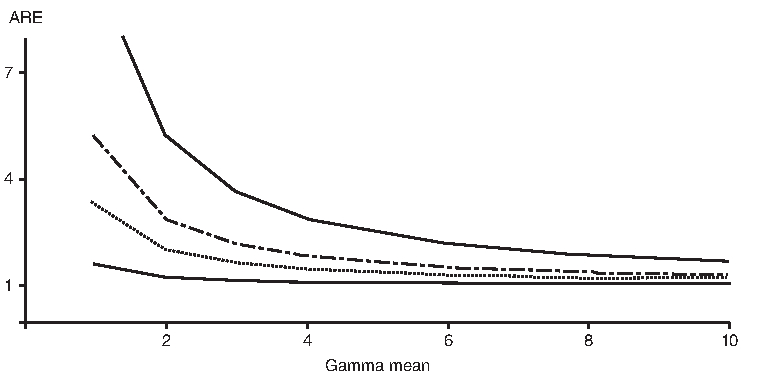
\includegraphics[width=.9\textwidth]{assets/chapter10/fig-10.1.1.pdf}
\caption{伽马均值的矩估计量与MLE的渐近相对效率. 四条曲线对应尺度参数值$(1,3,5,10)$，较高的曲线对应较大的尺度参数.}\label{fig:10.1.1}
\end{figure}\par
自助法由Efron于20世纪70年代末提出，最初的思想见Efron（\hyperref[bib:source106]{1979a}\hyperref[bib:source107]{b}），随后有专著\hyperref[bib:source108]{Efron（1982）}. 较新的思考与发展另见\hyperref[bib:source109]{Efron（1998）}.

先看一个其实并不需要自助法的简单例子.

\begin{example}[方差的自助法]\label{ex:10.1.19}\index{SI0095@非参数}\index{SI0913@重抽样}\index{SI0950@有放回}
在\autoref{ex:1.2.20}中，我们从四个数
$$2,4,9,12$$
中有放回地抽取四个数，计算所有可能的平均值. 这是最简单形式的自助法，有时称为非参数自助法（nonparametric bootstrap）. \autoref{fig:1.2.2}以直方图显示这些值.

所构造的是样本均值可能取值的重抽样. 已经看到，有$\binom{4+4-1}{4}=35$个不同的可能值，但它们并不等概率（所以不能视为随机样本）. $4^4=256$个（不全相异的）重抽样等可能，可以视为随机样本. 对第$i$个重抽样，令$\bar x_i^*$为其均值. 则样本均值$\bar X$的方差可估计为
\begin{equation}\label{eq:10.1.9}
\operatorname{Var}^*(\bar X)=\frac1{n^n-1}\sum_{i=1}^{n^n}(\bar x_i^*-\bar{\bar x}^{\,*})^2,
\end{equation}
其中$\bar{\bar x}^{\,*}=\frac1{n^n}\sum_{i=1}^{n^n}\bar x_i^*$是各个重抽样的均值. （通常以记号$*$表示自助法所得的、即重抽样所得的值.）

在本例中，自助法均值和方差分别为$\bar{\bar x}^{\,*}=6.75$和$\operatorname{Var}^*(\bar X)=3.94$. 事实表明，就均值和方差而言，自助法估计与通常估计几乎相同（见\autoref{exercise:10.13}）.
\end{example}

\sourcepageanchor{418}
我们已经看到如何计算自助法标准误，不过是在一个实际上不需要它的问题中. 自助法真正的优势在于，与Delta方法一样，方差公式\eqref{eq:10.1.9}几乎适用于任何估计量. 因此，对任意估计量$\hat\theta(\boldsymbol x)=\hat\theta$，可写为
\begin{equation}\label{eq:10.1.10}
\operatorname{Var}^*(\hat\theta)=\frac1{n^n-1}\sum_{i=1}^{n^n}(\hat\theta_i^*-\bar{\hat\theta}^{\,*})^2,
\end{equation}
其中$\hat\theta_i^*$是从第$i$个重抽样计算的估计量，$\bar{\hat\theta}^{\,*}=\frac1{n^n}\sum_{i=1}^{n^n}\hat\theta_i^*$是重抽样值的均值.

\begin{example}[二项方差的自助法]\label{ex:10.1.20}
在\autoref{ex:10.1.15}中，用Delta方法估计$\hat p(1-\hat p)$的方差. 对样本量$n$，也可将这个方差估计为
$$\operatorname{Var}^*(\hat p(1-\hat p))=\frac1{n^n-1}\sum_{i=1}^{n^n}\left((\hat p(1-\hat p))_i^*-\overline{\hat p(1-\hat p)}^{\,*}\right)^2.$$
\end{example}

但出现了新问题. 在\autoref{ex:10.1.19}中，$n=4$，自助法求和有256项. 对更典型的样本量，这个数会大到无法计算. （当$n>15$时，枚举全部可能的重抽样几乎不可能，至少对作者们如此.）不过，现在记起我们是统计学家：对重抽样再抽样即可.

因此，对样本$\boldsymbol x=(x_1,x_2,\ldots,x_n)$及估计$\hat\theta(x_1,x_2,\ldots,x_n)=\hat\theta$，选取$B$个重抽样（或自助样本，bootstrap samples），并计算
\begin{equation}\label{eq:10.1.11}\index{SI0913@重抽样}
\operatorname{Var}_B^*(\hat\theta)=\frac1{B-1}\sum_{i=1}^B(\hat\theta_i^*-\bar{\hat\theta}^{\,*})^2.
\end{equation}

\begin{example}[\autoref{ex:10.1.20}的结尾]\label{ex:10.1.21}
对样本量$n=24$，取$B=1{,}000$，计算$\hat p(1-\hat p)$的Delta方法方差估计和自助法方差估计. 当$\hat p\ne1/2$时，采用\autoref{ex:10.1.15}的一阶Delta方法方差估计；当$\hat p=1/2$时，采用\autoref{thm:5.5.26}的二阶方差估计（见\autoref{exercise:10.16}）. \autoref{tab:10.1.1}显示，在所有情形下，自助法方差估计都更接近真实方差，而Delta方法方差都低估了它. （这不应令人意外，因为\eqref{eq:10.1.7}表明Delta方法方差估计基于一个下界.）\footnote{译注：表中“真实值”与所述$n=24$二项模型不符. 按该模型对$Y=0,\ldots,24$逐项求和，$\operatorname{Var}[(Y/24)(1-Y/24)]$在$p=1/4,1/2,2/3$时约为$.001911,.000208,.001109$，并非表中的$.00484,.00531,.00519$. 原表及其比较结论保留；此核算仅针对表述的这三个参数值.}

\par\begin{table}[htbp]
\centering
\caption{$\hat p(1-\hat p)$的自助法（上行）与Delta方法（下行）方差. 当$\hat p=1/2$时使用二阶Delta方法（见\autoref{thm:5.5.26}）. 真实方差在假设$\hat p=p$下数值计算.}\label{tab:10.1.1}
\begin{tabular}{lrrr}\toprule
&$\hat p=1/4$&$\hat p=1/2$&$\hat p=2/3$\\\midrule
自助法&.00508&.00555&.00561\\
Delta方法&.00195&.00022&.00102\\\midrule
真实值&.00484&.00531&.00519\\\bottomrule
\end{tabular}
\end{table}\par

Delta方法是“一阶”近似，因为它基于泰勒级数展开的第一项. 当该项为零（例如$\hat p=1/2$）时，必须使用二阶Delta方法. 相比之下，自助法常有“二阶”准确性，能使展开中的不止第一项正确（见\hyperref[sec:10.6.3]{杂录10.6.3}）. 所以这里，自助法会自动修正$\hat p=1/2$的情形. （注意$24^{24}\approx1.33\times10^{13}$，这是极大的数，所以无法生成全部自助样本.）\footnote{译注：原文数值为$1.33\times10^{13}$，但$24^{24}\approx1.33\times10^{33}$. 保留原值；两者均支持这里无法枚举全部样本的结论.}
\end{example}

迄今讨论的自助法称为非参数自助法，因为没有假设总体pdf的函数形式.\index{SI0096@参数}\semanticindexanchor{96:418} 相比之下，也可以有参数自助法（parametric bootstrap）.

\sourcepageanchor{419}
假设样本$X_1,X_2,\ldots,X_n$来自pdf为$f(x\mid\theta)$的分布，其中$\theta$可以是参数向量. 可以用MLE $\hat\theta$估计$\theta$，并抽取样本
$$X_1^*,X_2^*,\ldots,X_n^*\sim f(x\mid\hat\theta).$$
若抽取$B$个这样的样本，就能用\eqref{eq:10.1.11}估计$\hat\theta$的方差. 注意，这些样本并非对数据的重抽样，而是从$f(x\mid\hat\theta)$实际抽出的随机样本；这个分布有时称为代入分布（plug-in distribution）.

\begin{example}[参数自助法]\label{ex:10.1.22}
假设有样本
$$-1.81,0.63,2.22,2.41,2.95,4.16,4.24,4.53,5.09,$$
其$\bar x=2.71$，$s^2=4.82$. 若假设基础分布为正态分布，则参数自助法会抽取样本
$$X_1^*,X_2^*,\ldots,X_n^*\sim\mathrm n(2.71,4.82).$$
基于$B=1000$个样本，算得$\operatorname{Var}_B^*(S^2)=4.33$. 根据正态理论，$S^2$的方差为$2(\sigma^2)^2/8$，可以用MLE $2(4.82)^2/8=5.81$估计它. 数据值模拟自方差为4的正态分布，因此这里参数自助法给出更好的估计. （在\autoref{ex:5.6.6}中，我们已经用现在所知的参数自助法估计过$S^2$的分布.）\footnote{译注：这里把以$s^2=4.82$代入的方差估计称为MLE；一般正态模型的方差MLE为$(n-1)s^2/n$，故该称呼与通常MLE定义不符. 原书数值与称呼均保留.}
\end{example}

现在有了一种计算标准误的通用方法，如何知道它是好方法呢？在\autoref{ex:10.1.21}中，它似乎优于Delta方法，而后者已知具有一些良好性质. 特别是，基于最大似然估计的Delta方法通常产生相合估计量. 对自助法能作相同的断言吗？

虽然无法十分一般地回答这个问题，但可以说，在许多情形下，自助法的确提供合理且相合的估计量.

为更精确，将计算自助法估计量的两个不同部分分开.
\begin{enumerate}[label=\alph*.]
\item\label{item:10.1.bootstrap.a} 证明当$B\to\infty$时，\eqref{eq:10.1.11}收敛到\eqref{eq:10.1.10}，即
$$\operatorname{Var}_B^*(\hat\theta)\xrightarrow{B\to\infty}\operatorname{Var}^*(\hat\theta).$$
\item\label{item:10.1.bootstrap.b}\index{SI0773@相合的自助法} 证明使用全部自助样本的估计量\eqref{eq:10.1.10}相合，即
$$\operatorname{Var}^*(\hat\theta)\xrightarrow{n\to\infty}\operatorname{Var}(\hat\theta).$$
\end{enumerate}
\hyperref[item:10.1.bootstrap.a]{(a)部分}可由大数定律建立（\autoref{exercise:10.15}）. 还应注意，\hyperref[item:10.1.bootstrap.a]{(a)部分}全部发生在样本内部. （\hyperref[bib:source199]{Lehmann，1999}，第6.5节把$\operatorname{Var}_B^*(\hat\theta)$称为近似器，而不是估计量.）

证明\hyperref[item:10.1.bootstrap.b]{(b)部分}稍微微妙一些，相合性正是在这里建立的. 独立同分布抽样时通常能够得到相合性，但在更一般的情形中未必如此（\hyperref[bib:source199]{Lehmann，1999}，第6.5节给出一个例子）. 关于相合性的更多细节（必然需要较高深的层次），见\hyperref[bib:source288]{Shao和Tu（1995}，第3.2.2节）或\hyperref[bib:source287]{Shao（1999}，第5.5.3节）.
